% !TEX root = ../diary-book.tex

\section{令和7年08月22日 一次宇宙線頻度}

Particle Data Groupの編纂では宇宙線の到来頻度は以下のような図になっている。

\begin{figure}[H]
\centering
   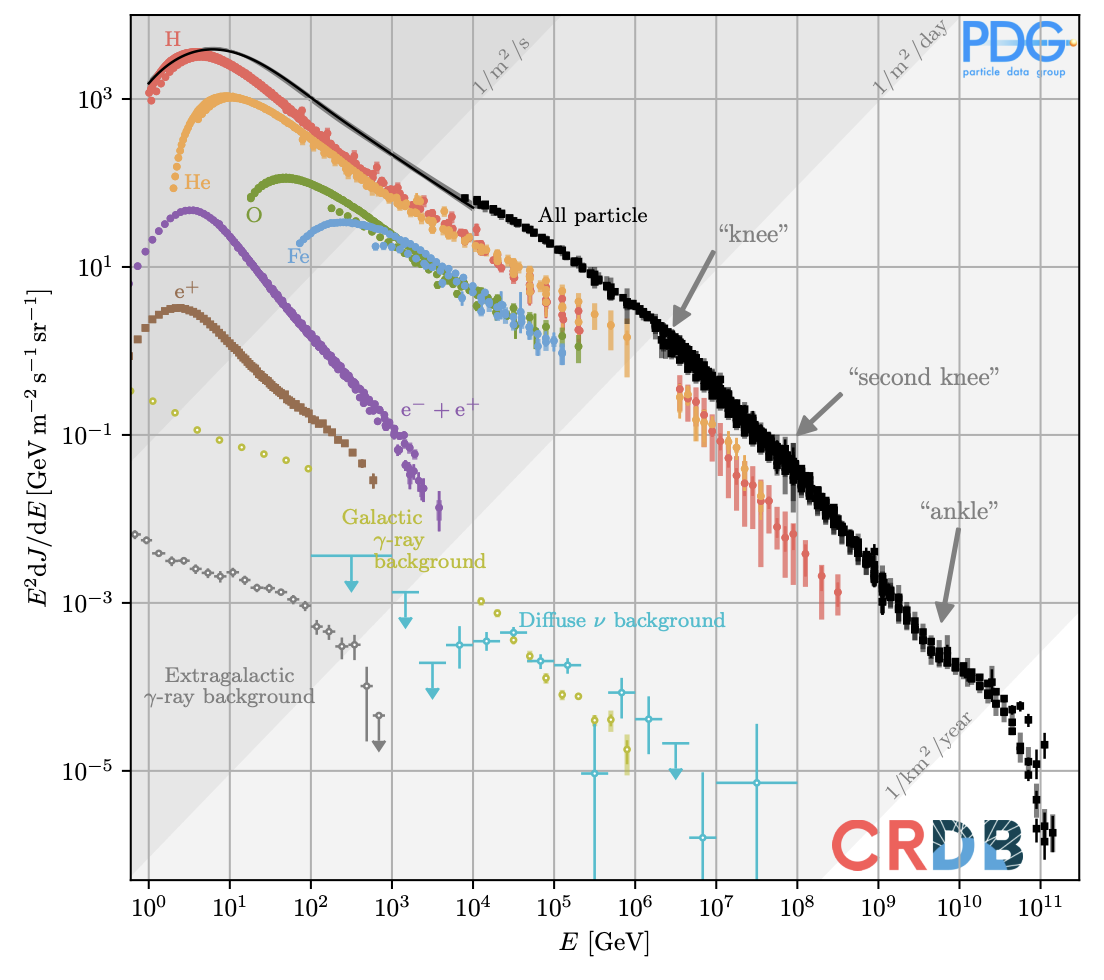
\includegraphics[width=.7\linewidth]{../../figs/CRDB/20250822-PDG-Fig30-1.png}
   \caption{Particle Data Groupの編纂による宇宙線の到来頻度。横軸はエネルギーの対数、縦軸は GeV あたり、単位面積当たり、単位立体角あたりの個数。}
   \label{fig:20250822-1}
\end{figure}

\href{https://lpsc.in2p3.fr/crdb/}{CRDB} から宇宙線（陽子）の到来頻度を抜き出してくる。

\begin{figure}[H]
  \begin{minipage}[b]{.48\linewidth}
    \centering
    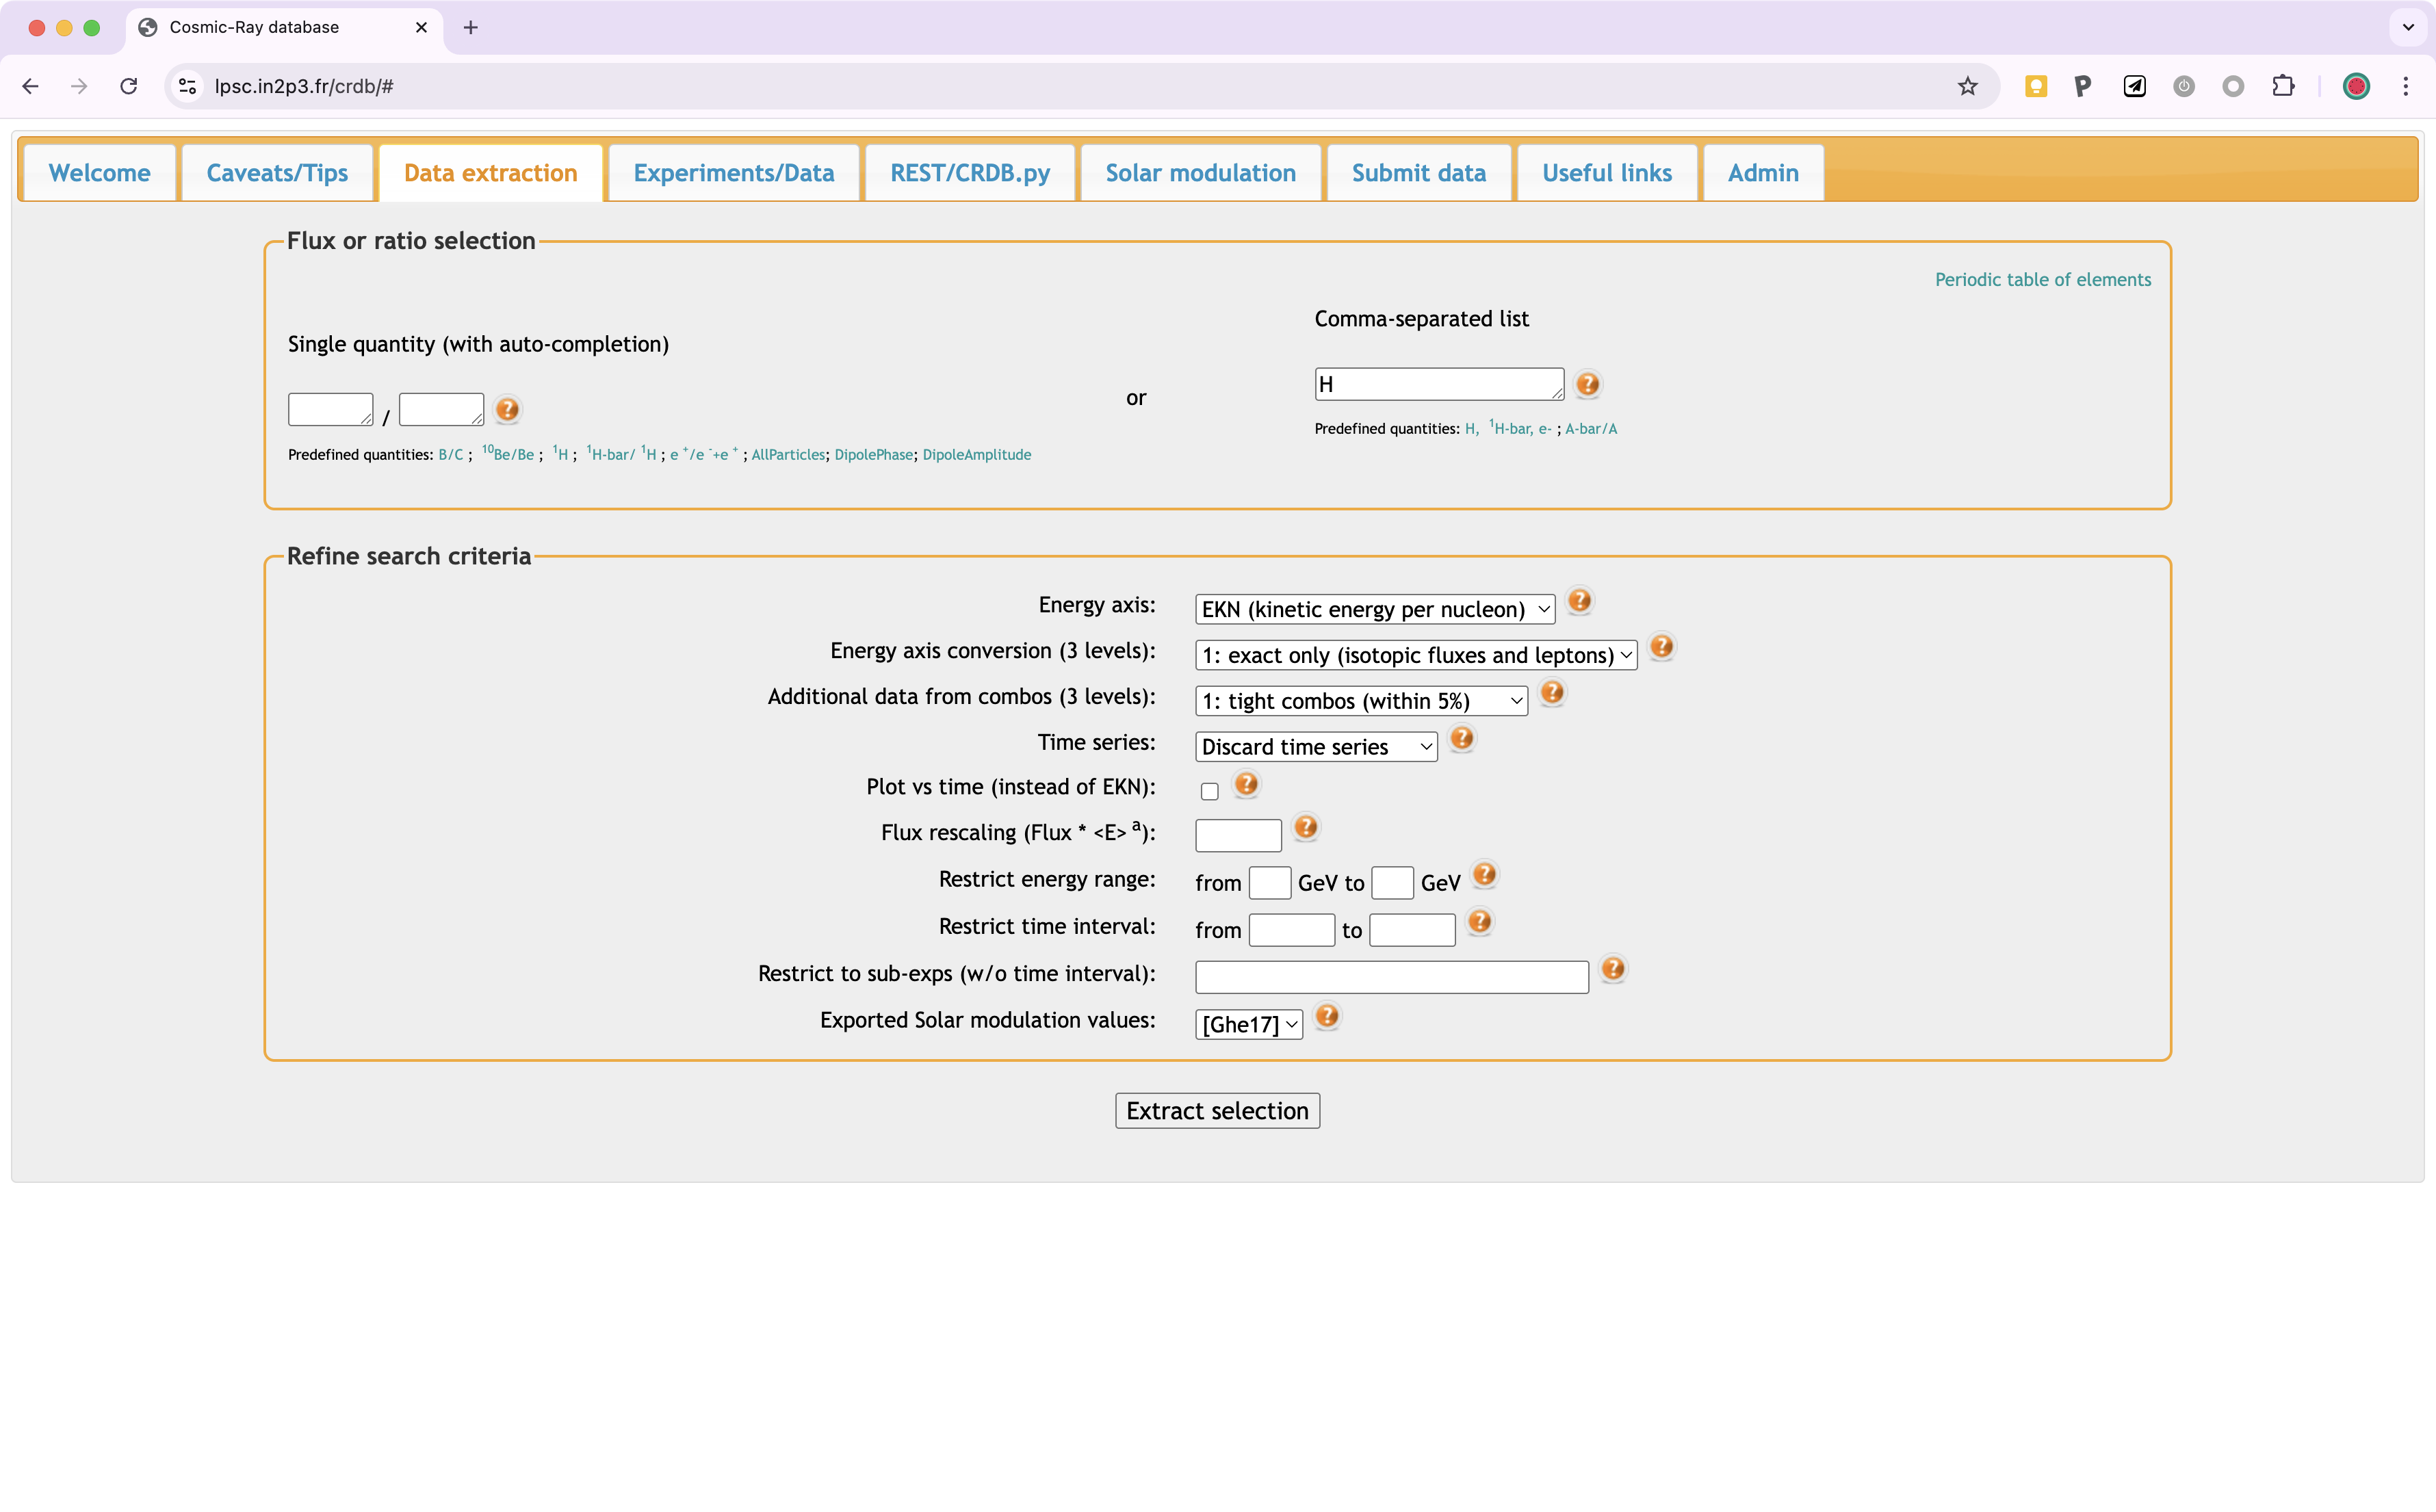
\includegraphics[width=.99\linewidth]{../../figs/CRDB/20250822-CRDB-Interface.png}
  \end{minipage}
  \begin{minipage}[b]{.48\linewidth}
    \centering
    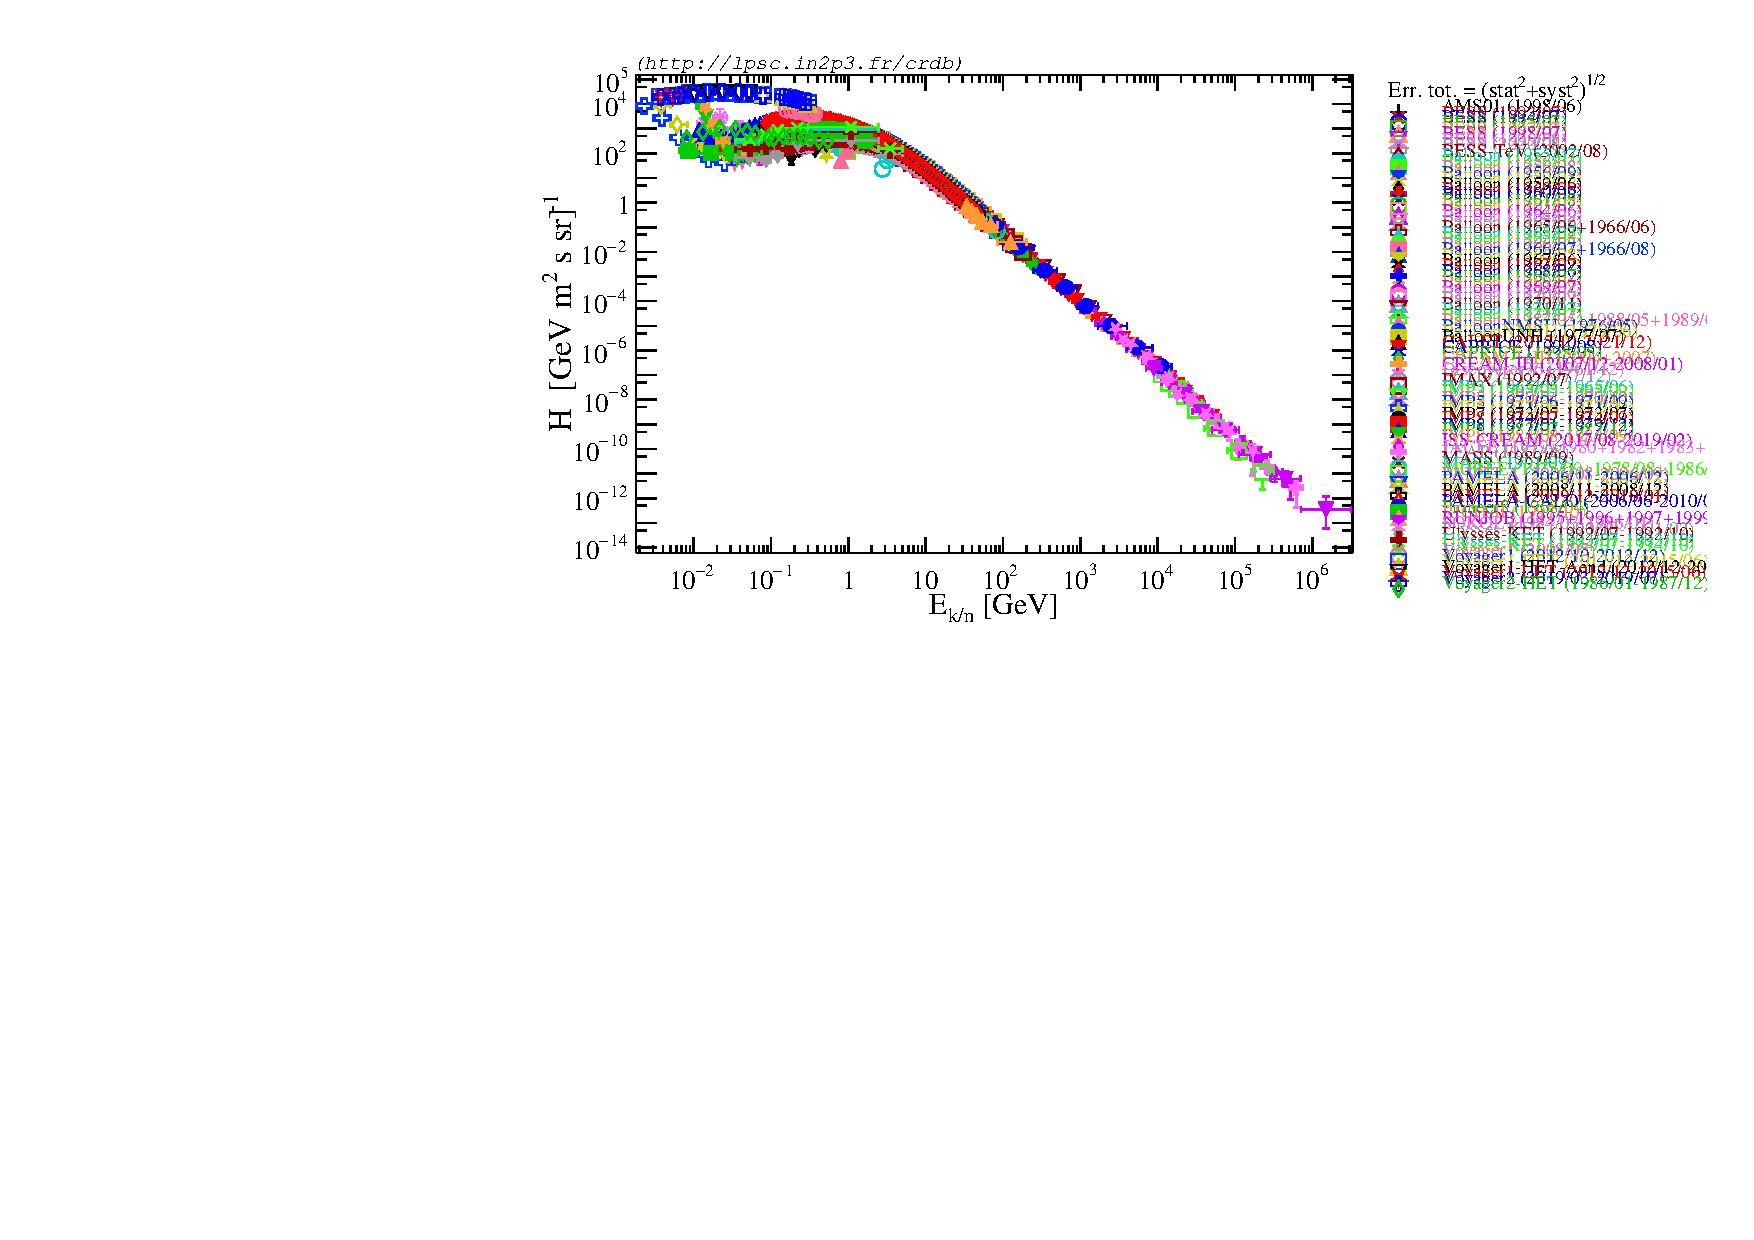
\includegraphics[width=.99\linewidth]{../../figs/CRDB/crdb_extracted.pdf}
  \end{minipage}
   \caption{CRDB のサイトで入力した値。左側の ratio のほうに 1H といれても 100 GeV 程度までしかデータがない。右側の Comma-separated list のほうに1Hといれると 1000~TeV までのデータが得られた。}
   \label{fig:20250822-1}
\end{figure}

\subsection{0.1~GeV以上に対する一次式と指数による近似}
2025-08-23 20:33:53 実施　

\begin{equation}
\log_{10}(\frac{dN}{dE d\Omega dt}) = (p0 + p1 \log_{10}(E)) * \exp(p2 \exp (- p3 (\log_{10}(E)-p4)))
\end{equation}

\begin{codebox}{一次式と指数による近似の結果}

  \begin{minted}{shell} 
****************************************
Minimizer is Minuit2 / Migrad
Chi2                      =  4.27391e+06
NDf                       =         1204
Edm                       =  2.33582e-09
NCalls                    =          156
p0                        =        4.088                         (fixed)
p1                        =       -2.703                         (fixed)
p2                        =    -0.637902   +/-   3.45444e-06 
p3                        =     0.988519   +/-   3.34817e-05 
p4                        =    -0.221478   +/-   1.73338e-06 
  \end{minted}
\end{codebox}


\begin{figure}[H]
   \centering
   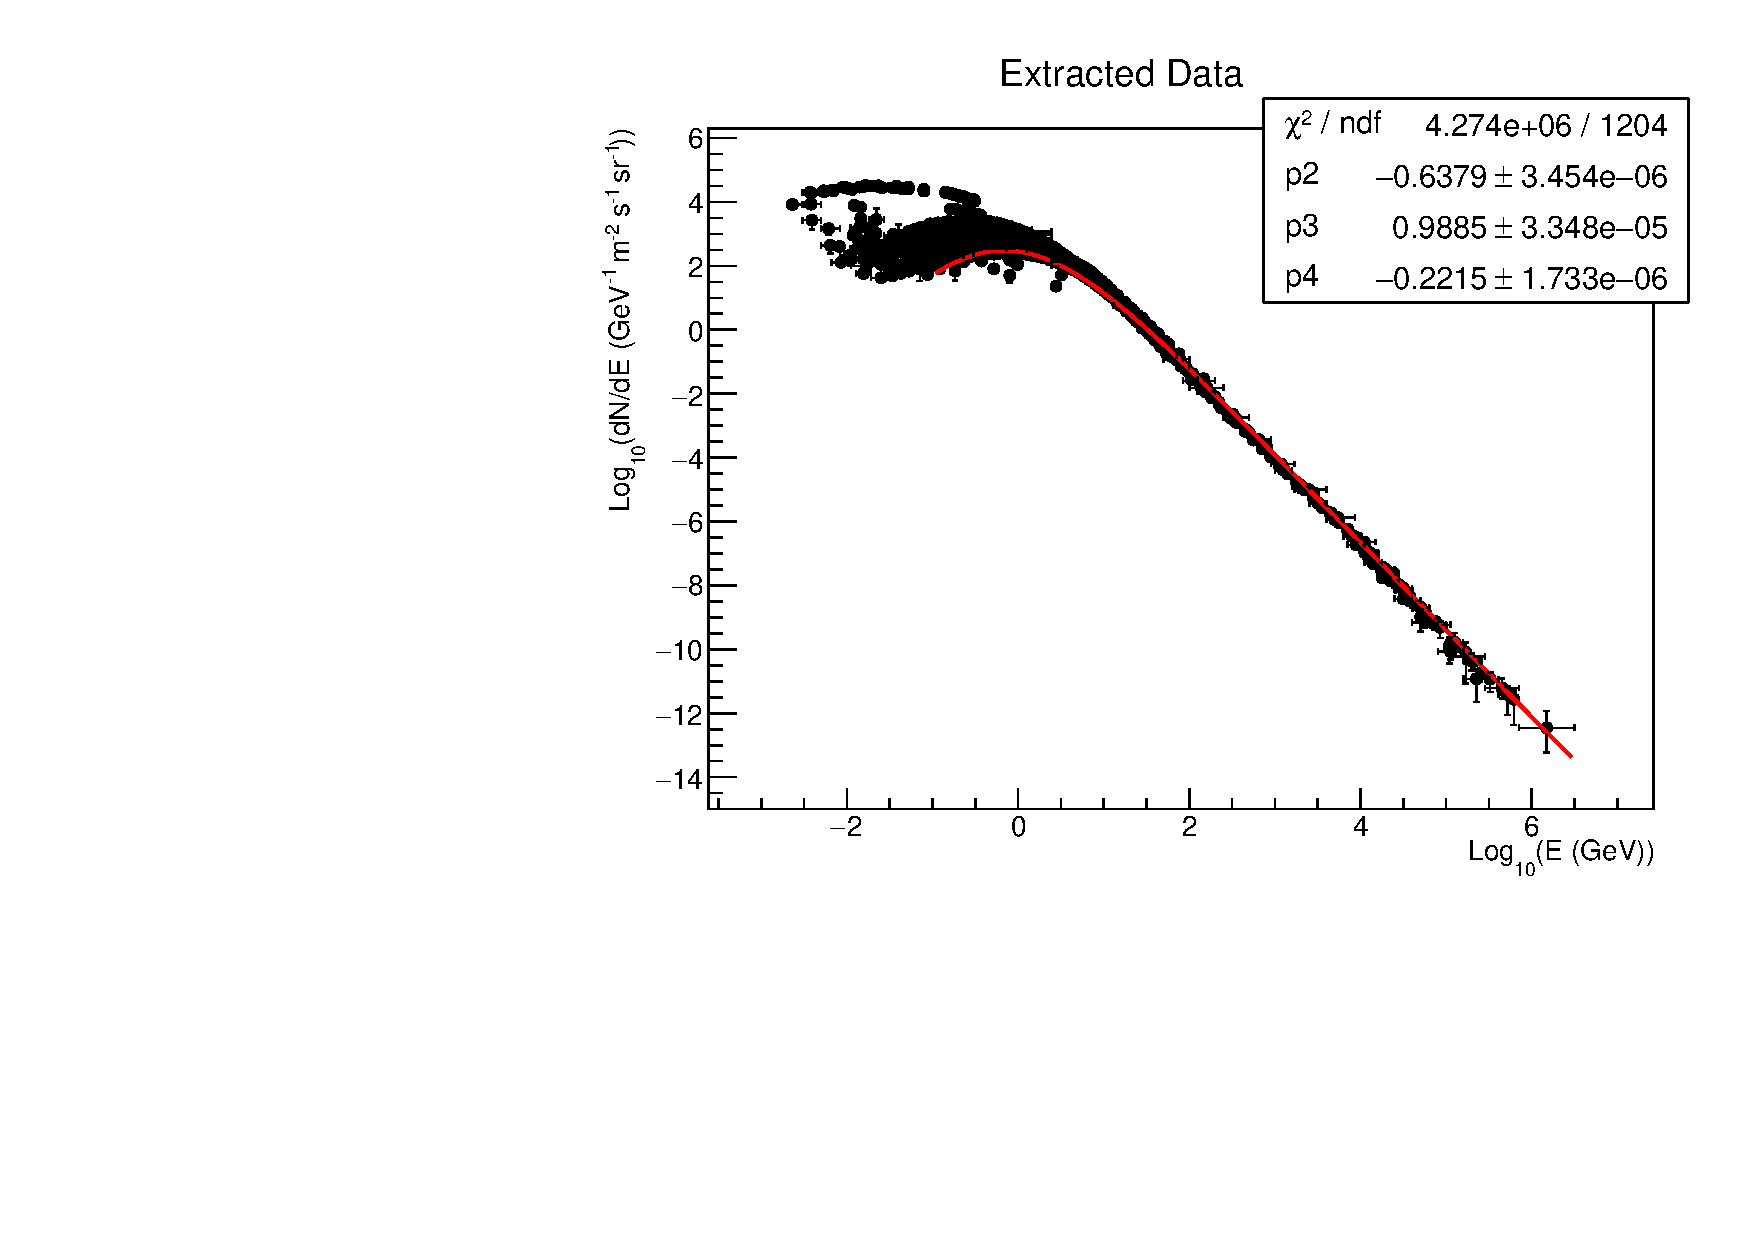
\includegraphics[width=.7\linewidth]{../../figs/CRDB/approx-wide.pdf}
   \caption{CRDB のデータを三次関数でフィッティングした結果。横軸はエネルギーの対数、縦軸は GeV あたり、単位面積当たり、単位立体角あたりの個数の対数。}
   \label{fig:20250822-3}
\end{figure}




\subsection{10~GeV以上に対する三次曲線による近似}
このデータを使って、近似曲線を得る。普通に fit しようとするとさすがに桁が合わないので、対数スケールでフィッティングを行う。エネルギー、強度ともに対数を取ったもののうち 1~GeV 以上のデータを使うことにする。三次関数くらいがちょうど良さそう。得られた数式は以下の通り。

\begin{equation}
   \log_{10}(\frac{dN}{dE d\Omega dt}) = 0.0028 \times (\log_{10}(E))^3 - 0.0652 \times (\log_{10}(E)^2 - 2.42761 \times \log_{10}(E) + 3.82585
\end{equation}

\begin{codebox}{フィッティングの結果}
  \begin{minted}{shell}
****************************************
Minimizer is Minuit2 / Migrad
Chi2                      =      450.404
NDf                       =          368
Edm                       =  2.01236e-06
NCalls                    =          302
p0                        =      3.82585   +/-   0.0618054   
p1                        =     -2.42761   +/-   0.0821447   
p2                        =   -0.0642256   +/-   0.0326427   
p3                        =   0.00279992   +/-   0.00401469   
    
  \end{minted}
\end{codebox}


\begin{figure}[H]
   \centering
   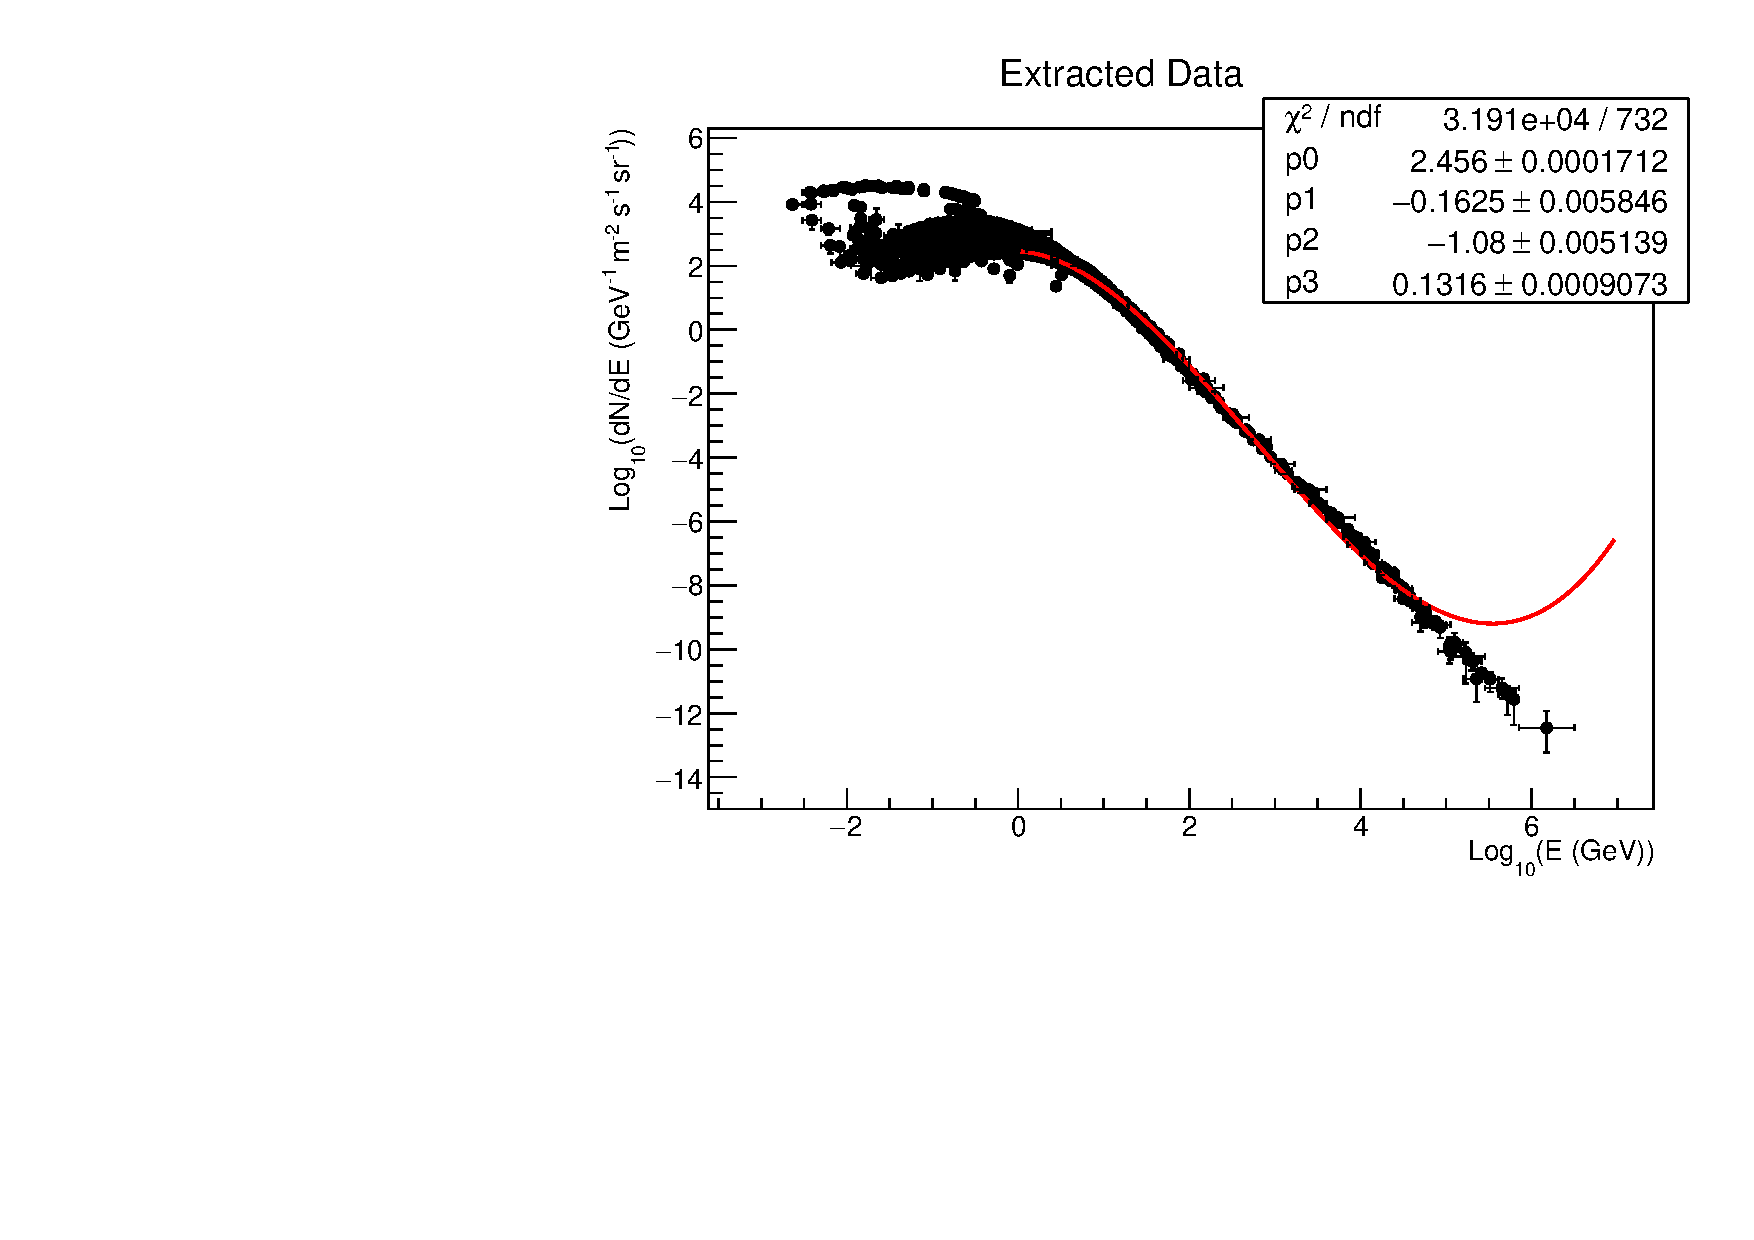
\includegraphics[width=.7\linewidth]{../../figs/CRDB/approx.pdf}
   \caption{CRDB のデータを三次関数でフィッティングした結果。横軸はエネルギーの対数、縦軸は GeV あたり、単位面積当たり、単位立体角あたりの個数の対数。}
   \label{fig:20250822-2}
\end{figure}

